% Kapitel 2 %

\section{Analoger Sensor: Der Temperatur-Sensor LM35 und LM36}
\label{sec:lm35}
Die Temperatursensoren LM35 und LM36 oder die Funktionsgleichen TMP35 TMP36 sind sogenannte analoge Sensoren. Analoge Sensoren haben meistens 3 PINs. Zwei PINs werden zur Spannungsversorgung (U$_S$ und GND) und einer PIN (V$_{out}$) für den Messwert benötigt. Dabei variiert die Spannung an V$_{out}$ linear mit 10mV pro $1^\circ$C\footnote{Eigentlich werden Temperaturunterschiede in Grad Kelvin K angegeben.}. Beim LM35 entspricht einer Spannung von 0mV dem Temperaturwert von $0^\circ$C. Da mit dem TMP36 auch negative Temperaturen gemessen werden können entspricht eine Spannung von 0mV ca. dem Temperaturwert -$50^\circ$C (siehe Abb. \ref{fig:daten-tmp36}). 
\begin{figure}[h]
  \begin{center}
  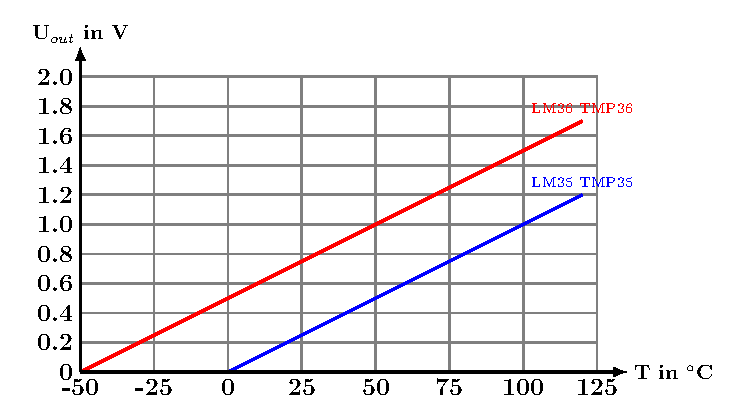
\includegraphics[width=0.55\textwidth]{Kapitel2/Tikz/lm35temp.pdf}
  \caption{Temperatur Ausgangsspannungs Verlauf des LM35}
  \label{fig:daten-tmp36}
  \end{center}
\end{figure}

\marginfigure{Kapitel2/Bilder/lm35}{PIN Belegung}{fig:lm35}

Solche Informationen erhält man aus einem sogenannten Datenblatt. Jeder Hersteller liefert ein mehr oder weniger ausführliches Datenblatt, das den Aufbau und die Funktion des Bauteils beschreibt. 
Für die Temperatursensoren kann anhand dieser Informationen eine Formel zur Berechnung des Temperaturwerts hergeleitet werden. Für den LM35 und TMP35 ergibt sich die Formel (\ref{eqn:lm35}) und für den LM36 und TMP36 die Formel (\ref{eqn:tmp36}):
\begin{multicols}{2}
\begin{equation}\label{eqn:lm35}
 T(V_{out}) = \frac{V_{out}}{10}
\end{equation}
\begin{equation}\label{eqn:tmp36}
 T(V_{out}) = \frac{V_{out} - 500}{10}
\end{equation}
\end{multicols}

\subsection{Der Beipiel-Sketch} 

Wenn zur Messung der Temperatur eine Verarbeitung der gemessenen Werte am analogen Eingang nötig sind, ist es für die Übersicht des Sketches sinnvoll, diese Berechnung in einer sog. Funktion auszulagern. Der Vorteil ist, dass wenn man den Sensor gegen einen anderen Sensor austauscht, bei dem die Messgröße anhand einer anderen Formel berechnet werden muss, dann findet die Anpassung nur in dieser Funktion statt.     

\begin{multicols}{2}
\begin{arduinoCode}{Testsketch ``TempTest'' für einen Temperatursensor LM35}{lst:temp}
int senPin = A0; (*@ \tikzmark{senPin} @*)
int VS = 5000;(*@ \tikzmark{vs} @*)
float temp = 0.0; 
 
void setup() {
  Serial.begin(9600);
}
 
void loop() {
  temp =  getTemperature(); (*@ \tikzmark{fktauf} @*)
  Serial.print( temp );
  Serial.println(" C");
}
 
float getTemperature() { 
  int senV = analogRead(senPin); 
  float t = map(senV,0,1023,0,VS)/10.0;(*@\tikzmark{funk_def} @*)
  return t;
}
\end{arduinoCode}

\vfill\null 
\columnbreak

\null\vfill
\begin{itemize}
  \itemsep15pt
    \item[] \tikzmarkcomment{item1}{Definition des Sensor PINs}
    \item[] \tikzmarkcomment{item2}{Versorgungsspannung in mV}
    \itemsep35pt
    \item[] \tikzmarkcomment{item3}{Die Funktion wird aufgerufen}
    \itemsep45pt
    \item[] \tikzmarkcomment{item4}{Definition der Funktion für  einen LM36 muss diese Zeile abgeändert werden: \\ \small{\textbf{float temp = (map(senV,0,1023,0,VS)-500)/10;}}}
\end{itemize}
\vfill \null

\begin{tikzpicture}[remember picture,overlay]
  \path[red, thick,-] (senPin.east) edge [out=0 , in=180] (item1);
  \path[red, thick,-] (vs.east) edge [out=0 , in=180] (item2);
  \path[red, thick,-] (fktauf.east) edge [out=0 , in=180] (item3);
  \path[red, thick,-] (funk_def.east) edge [out=0 , in=180] (item4);
\end{tikzpicture}


\end{multicols}

\marginfigure{Kapitel2/Bilder/temperatursensor}{Temperatursensor LM35CZ}{fig:temp}
\subsection{Aufgaben}

Baue die abgebildete Schaltung (Abb. \ref{fig:temp}) auf. Achte auf die Beschriftung und somit auf den richtigen Einbau des Temperatur-Sensors. Sollte sich der Temperatursensor, nachdem du den Arduino mit dem PC verbunden hast sehr schnell erwärmen, dann hast du den Sensor falsch eingebaut! Unterbreche die Verbindung zum PC und überprüfe den richtigen Einbau. Wenn der Temperatursenor sich zu sehr erwärmt, kann er zerstört werden! 
 
\subsubsection{Aufgabe 1}
Erstelle und lade den Beispiel-Sketch ``TempTest'' \ref{lst:temp} auf deinen Arduino und öffne dann die serielle Verbindung. Messe verschiedene Temperaturen.


\subsubsection{Aufgabe 2}
\margininfo{if ist eine bedingte Anweisung (siehe Kapitel \ref{sec:bedingte-Anweisung})}

Baue mit Hilfe des Temperatursensor und den drei LEDs (grün, gelb und rot) ein Thermometer bei dem bis zur 
Temperatur 20$^{\circ}$C nur die grüne LED leuchtet, bis 25$^{\circ}$C die grüne und gelbe LED leuchten und ab 30$^{\circ}$C die grüne, gelbe und rote LED leuchten. 
Füge dazu den Code in die loop()-Routine ein und ergänze entsprechend. In Kapitel \ref{sec:bedingte-Anweisung} erfährst du mehr über bedingte Anweisugen. 

\begin{arduinoCode}{}{}
if (temp > 20) {
  // gruen an, gelb rot aus
}
if (temp > 25) {
  // gruen gelb an, rot aus
}
if (temp > 30) {
  // gruen gelb rot an
}
\end{arduinoCode}


\subsubsection{Aufgabe 3 (Projekt)}%

In Amerika werden normalerweise Temperaturen in Fahrenheit $F$ angegeben. Die Umrechnung ist einfach: 
\begin{equation}
 F(T) = T\cdot 1.8 + 32
\end{equation}
Schreibe eine weiter Funktion getFahrenheit(), die die gemessene Temperatur in Fahrenheit berechnet. Übermittle mit Hilfe einer seriellen Verbindung den gemessenen Temperaturwert in Grad Celsius und Fahrenheit an den PC.

Die wichtigste Temperaturskala ist die Kelvin-Skala. Bei der Kelvin Skale entspricht die Temperatur am absoluten Nullpunkt 0K und bei $0^{\circ}$C umgerechnet 273,15K. 

Es gibt noch weitere Temperaturskalen. Suche in Wikipedia nach dem Schlagwort ``Temperaturskala''. Entwerfe weiter Unterprogramme für die Temperaturskalen: Kelvin und Rømer

\begin{multicols}{2}
\begin{arduinoCode}{}{}
float GetFahrenheit(int vs) { 
  int senV = analogRead(senPin); 
  float temp = (map(senV,0,1023,0,vs)-500)/10;
         (*@ \tikzmark{umrechnung} @*)   
  return fahrenheit;
\end{arduinoCode}
\vfill\null 
\columnbreak

\null\vfill
\begin{itemize}
  \itemsep15pt
    \item[] \tikzmarkcomment{item1}{Umrechnung von Grad Celsius nach Fahrenheit}
 \end{itemize}
\vfill \null

\begin{tikzpicture}[remember picture,overlay]
  \path[red, thick,-] (umrechnung.east) edge [out=0 , in=180] (item1);
\end{tikzpicture}
\end{multicols}

 
  
 
\sectionInformatik{C Sprachelemente: Unterprogramme}
Der Einsatz eines Unterprogramm ist sinnvoll, um das Programm übersichtlich zu halten. Wenn z.B. das Auslesen und Berechnen einer Messgröße eines Sensors aufwendig ist, wird der Sketch übersichtlicher, wenn dieser Teil des Programms aus der loop()-Routine in ein eigenes Unterprogramm ausgelagert wird. Unterprogramme werden dann unverzichtbar, wenn einzelne Programmteile sich wiederholen. Wenn diese Teile nicht in ein Unterprogramm ausgelagert werden und später Änderungen vorgenommen werden, dann müssen diese Änderungen an verschiedenen Stellen vorgenommen werden. Wenn ein Unterprogramm benutzt wird, muss nur an einer einzigen Stelle etwas verändert werden!

\margininfo{Don’t repeat yourself -- DRY}

\subsection{Allgemeiner Aufbau eines Unterprogrammes in C}

Ein Unterprogramm besteht aus zwei Teilen: einem Kopf und einen Körper. Im Kopf wird der Typ, der Name und eventuelle Eingabeparameter festgelegt. Der Körper besteht aus den eigentlichen Anweisungen und einem eventuellen Rückgabewert.
\begin{multicols}{2}
\null\vfill
\begin{arduinoCode}{Aufbau eines Unterprogrammes}{lst:c-function}
  (*@ \tikzmark{fktTyp} @*)        (*@ \tikzmark{fktParameter} @*)
type Name(parameter){
       (*@ \tikzmark{fktName} @*)
    
  (*@ \tikzmark{fktBody} @*)  


  return rueckgabeWert; (*@ \tikzmark{fktReturn} @*)
}           
\end{arduinoCode}
\vfill\null 
\columnbreak
\vfill\null 
\begin{itemize}
  \itemsep15pt
    \item[] \tikzmarkcomment{item1}{Unterprogramm Type: z.B. int oder boolean}
    \item[] \tikzmarkcomment{item2}{Parameter: ein Wert, der übergeben wird}
    \item[] \tikzmarkcomment{item3}{Name des Unterprogramm}
    \item[] \tikzmarkcomment{item4}{Unterprogramm Code}
    \item[] \tikzmarkcomment{item5}{Rückgabewert: Wert der zurückgegeben wird}
 \end{itemize}
\vfill \null

\begin{tikzpicture}[remember picture,overlay]
  \path[red, thick,-] (fktTyp.east) edge [out=25 , in=180] (item1);
  \path[red, thick,-] (fktParameter.east) edge [out=25 , in=180] (item2);
  \path[red, thick,-] (fktName.east) edge [out=-15 , in=180] (item3);
  \path[red, thick,-] (fktBody.east) edge [out=0 , in=180] (item4);
  \path[red, thick,-] (fktReturn.east) edge [out=0 , in=180] (item5);
\end{tikzpicture}
\end{multicols}


Unterprogramme können anhand ihres Types unterschieden werden. So kann man Unterprogramme ohne Rückgabewert Prozeduren und Unterprogramme mit Rückgabewert Funktionen nennen.
\margininfo{In vielen Programmiersprachen werden die Begriffe Unterprogramm und Funktion synonym verwendet.}

\subsection{Unterprogramm ohne Rückgabewert -- Prozeduren}
Unterprogramme die keinen Rückgabewert haben, werden Prozeduren genannt. Du solltest zwei Prozeduren schon gut kennen: Die setup()- und loop()-Prozeduren. Das Type-Schlüsselwort ist void (eng. für leer). 

\subsubsection{Beispiel: Die Reset()-Prozedur}
Manchmal ist es sinnvoll den Arduino Softwaretechnisch neu zu starten. Eine einfache Lösung stellt die Verwendung des Reset-PINs dar. Wenn am Reset-PIN HIGH anliegt wird der Arduino neue gestartet. Dies kann zum Beispiel mit einem Push-Buttom realisiert werden, oder mit Hilfe eines digitalen PINs.

\marginfigure{Kapitel2/Bilder/reset.png}{Reset Prozedure}{fig:reset}

\begin{multicols}{2}
\null\vfill
\begin{arduinoCode}{Reset()-Prozedur}{lst:reset}
  (*@ \tikzmark{fktTyp} @*)
void Reset() (*@ \tikzmark{fktName} @*)
{      
  int resetPin=12;
  pinMode(resetPin, OUTPUT);     (*@ \tikzmark{fktBody} @*)  
  digitalWrite(resetPin, HIGH);    
}
\end{arduinoCode}

\vfill\null 
\columnbreak
\vfill\null 
\begin{itemize}
  \itemsep20pt
    \item[] \tikzmarkcomment{item1}{\textbf{void} bedeutet, dass die Prozedur keine Rückgabewert hat}
    \item[] \tikzmarkcomment{item2}{Name des Unterprogramm}
    \item[] \tikzmarkcomment{item3}{Der Arduino wird mit Hilfe des Reset-PINs und PIN 12 neu gestartet}
 \end{itemize}
\vfill \null

\begin{tikzpicture}[remember picture,overlay]
  \path[red, thick,-] (fktTyp.east) edge [out=25 , in=180] (item1);
  \path[red, thick,-] (fktName.east) edge [out=0 , in=180] (item2);
  \path[red, thick,-] (fktBody.east) edge [out=0 , in=180] (item3);
\end{tikzpicture}
\end{multicols}

Es gibt Lösungen ohne die Verwendung des Reset-PINs. Wenn man mit den Schlagwörtern Watchdog und Reset Function sucht, findet man schnell solche Lösungen. Aber es ist Vorsicht geboten, wenn eine solche Reset-Prozedure zu schnell aufgerufen wird, startet der Arduino neue bevor der Bootloader einen neuen Sketch aufspielen kann. Damit wird der IC unbrauchbar und muss ausgetauscht werden.    

\pagebreak
\subsection{Unterprogramm mit Rückgabewert -- Funktion}
Unterprogramme werden als Funktion bezeichnet, wenn sie einen Wert zurückliefen.

\subsubsection{Beispiel: }

Oft wird die Zeit benötigt, die ein Taster gedrückt wird. Es gibt zwar einen Arduino Befehl dafür (pulseIn()), aber durch die Verwendung einer Funktion wird der Sketch übersichtlicher.  

\begin{multicols}{2}
\null\vfill
\begin{arduinoCode}{ pushedTime()-Funktion }{lst:pushedTime}
  (*@ \tikzmark{fktTyp} @*)
int pushedTime()  (*@ \tikzmark{fktName} @*)
{       
  return pulseIn(pushPIN, HIGH); (*@ \tikzmark{fktReturn} @*)
  
}
\end{arduinoCode}

\vfill\null 
\columnbreak
\vfill\null 
\begin{itemize}
  \itemsep15pt
  \item[] \tikzmarkcomment{item1}{Der Rückgabewert ist vom Type \textbf{integer}}
  \item[] \tikzmarkcomment{item2}{Name des Unterprogramm}
  \item[] \tikzmarkcomment{item3}{Rückgabewert: Wert der zurückgegeben wird}
 \end{itemize}
\vfill \null

\begin{tikzpicture}[remember picture,overlay]
  \path[red, thick,-] (fktTyp.east) edge [out=25 , in=180] (item1);
  \path[red, thick,-] (fktName.east) edge [out=0 , in=180] (item2);
  \path[red, thick,-] (fktReturn.east) edge [out=0 , in=180] (item3);
\end{tikzpicture}
\end{multicols}


\subsection{Unterprogramm mit Parameter}

Parameter können an das Unterprogramm übermittelt werden,
so ist es möglich, dass Informationen von Hauptprogramm zum Unterprogramm übermittelt werden.  

\clearpage
\begin{multicols}{2}
\null\vfill
\begin{arduinoCode}{ blinkLED()-Parameter }{lst:reset}
  (*@ \tikzmark{fktTyp} @*)     (*@ \tikzmark{fktName} @*)         (*@ \tikzmark{fktParameter} @*)
void blinkLED(int ledPIN)
{
  pinMode(ledPIN, OUTPUT);    
  digitalWrite(ledPIN, HIGH);
  delay(1000);                  (*@ \tikzmark{fktBody} @*)
  digitalWrite(ledPIN, LOW);
  delay(1000);  
}
\end{arduinoCode}
\vfill\null 
\columnbreak
\vfill\null 
\begin{itemize}
  \itemsep15pt
    \item[] \tikzmarkcomment{item1}{\textbf{void} also keine Rückgabewert}
    \item[] \tikzmarkcomment{item2}{Name des Unterprogramm}
    \item[] \tikzmarkcomment{item3}{Parameter: digitaler PIN}
    \item[] \tikzmarkcomment{item4}{Eine LED am blinkt mit einer Sekunde}
 \end{itemize}
\vfill \null

\begin{tikzpicture}[remember picture,overlay]
  \path[red, thick,-] (fktTyp.east) edge [out=25 , in=180] (item1);
  \path[red, thick,-] (fktName.east) edge [out=15 , in=180] (item2);
  \path[red, thick,-] (fktParameter.east) edge [out= 5 , in=180] (item3);
  \path[red, thick,-] (fktBody.east) edge [out=0 , in=180] (item4);
\end{tikzpicture}
\end{multicols}

\subsection{Aufgaben:}

\subsubsection{Aufgabe 1:}

Du hast jetzt schon einige Arduino Befehle kennengelernt und in deiner Befehlsübersicht dokumentiert! Ordne die Befehle, die Unterprogramme sind in einer Tabelle. Unterscheide die Befehle nach Prozedur, Funktion und Unterprogramme mit Parameter. Einzelne Befehle können auch in mehrmals auftauchen. In Abb. \ref{tab:unterprogramme} ein.

\begin{figure}[h]
  \begin{center}
  \tikzset{ 
      table/.style={
          matrix of nodes,
          row sep=-\pgflinewidth,
          column sep=-\pgflinewidth,
          nodes={
              rectangle,
              draw=black,
              align=center
          },
          minimum height=1.5em,
          text depth=0.5ex,
          text height=2ex,
          nodes in empty cells,
  %%
          every even row/.style={
              nodes={fill=gray!20}
          },
          column 1/.style={
              nodes={text width=0.3\textwidth}
          },
          column 2/.style={
              nodes={text width=0.6\textwidth, align=left}
          },
          row 1/.style={
              nodes={
                  fill=black!80,
                  text=white,
                  align=center,
                  font=\bfseries
              }
          }
      }
  }
  \begin{tikzpicture}
  \matrix (first) [table,text width=6em]
  {   
   Unterprogramm Typ:   & Arduino Befehle \\
   Prozeduren       &  setup() \\
   Funktion         &  digitalRead(PIN) \\
   Unterprogramm mit Parameter &  delay(1000) \\
  };
  \end{tikzpicture}
  \caption{Arduino Befehle sind Unterprogramme}
  \label{tab:unterprogramme}
  \end{center}
\end{figure}

\subsubsection{Aufgabe 2: Der SOS-Sketch mit Unterprogrammen} 

In Kapitel 1 hast du den Sketch ``SOS'' geschrieben, der mit Hilfe einer LED an PIN 10 den Morsecode SOS (kurz kurz kurz, lang lang lang, kurz kurz kurz) optisch sendet. Öffne diesen Sketch und analysiere ihn. Zwei Sachverhalte wirst du wahrscheinlich feststellen:

\begin{itemize}
\item[1.] Du wirst Schwierigkeiten haben deinen Sketch schnell zu verstehen! 
\item[2.] Wenn du die Zeiten für die lange Leuchtdauer verdoppeln möchtest, dann muss du das an sehr vielen Stellen machen. 
\end{itemize}

Der Sketch ist unübersichtlich, da sehr oft hintereinander sehr ähnlicher Code steht. Mit Hilfe der Prozeduren lang() und kurz() dann die loop()-Methode vereinfacht werden. Füge den Beispielcode aus Listing \ref{lst:lang_kurz} nach der loop()-Methode in den Sketch ein und vervollständige die Prozedur kurz(). Ersetzt in deiner loop()-Methode den jeweiligen Code durch den Aufruf der Prozedur kurz() oder lang() (siehe Listing \ref{lst:lang_kurz}). 

\begin{multicols}{2}
\null\vfill
 
\begin{arduinoCode}{ Die Prozeduren lang() und kurz() }{lst:lang_kurz}
void lang() {
  // led soll 2 Sekunden leuchten
  digtialWrite(10, HIGH);
  delay(2000);
  digtialWrite(10, LOW);
  delay(1000);
}

void kurz() {
  // led soll 1 Sekunden leuchten
}  
\end{arduinoCode}
\vfill\null 
\columnbreak
\vfill\null 
\begin{arduinoCode}{ Die Prozeduren blink(int time) }{lst:blink_mit_parameter}
void blink(int time) {
  digtialWrite(10, HIGH);
  delay(time);
  digtialWrite(10, LOW);
  delay(1000);
}
\end{arduinoCode}
\end{multicols}

Jetzt sollte deine loop()-Prozedur schon viel einfacher aussehen. Aber eigentlich machen deine beiden Prozeduren, mehr oder wenige das selbe. Erstelle jetzt eine Prozedur blink() mit dem Parameter time (siehe Listing \ref{lst:blink_mit_parameter}). Vereinfache deinen Sketch weiter und dokumentier ihn ausführlich.

\clearpage
\section{Widerstände und Spannungsteiler}
\label{sec:spannungsteiler}
Würde man einen digitalen Pin mit 5 Volt verbinden, so läge (wenn der digitale Pin auf INPUT gestellt ist) der Zustand ``HIGH'' an. Auf der anderen Seite, den nun GND mit dem digitalen Pin verbunden wäre, so läge der Zustand ``LOW'' an. Was wäre, wenn man den digitalen Pin sowohl mit 5Volt und mit GND verbindet? Ist der anliegende Zustand dann ``HIGH``oder ``LOW''? Leider würde es einen Kurzschluss geben, da 5 Volt direkt mit GND verbunden wäre, und kein Strombegrenzer (LED mit Vorwiderstand, Lautsprecher, Motor oder ähnliches) vorhanden ist, steigt der Strom soweit an, bis er über den maximal zulässige Strom von 500mA liegt. Der Spannungsregler wird überhitzen und sich hoffentlich rechtzeitig abschalten, bevor etwas kaputt geht. 

Interessanter wird es, wenn man die beiden Verbindungen vom digitalen Pin zu GND bzw. vom digitalen Pin zu 5V jeweils mit Widerständen verbindet. So entsteht kein Kurzschluss, da nur ein schwacher Strom durch die beiden Widerstände am Mikrocontroller vorbei fließt. Diese Schaltung bezeichnet man als Spannungsteiler (siehe Abb. \ref{fig:spannungsteiler}).

\margintikzfig{\begin{circuitikz} \draw
 (0,0) node[anchor=east]{GND}
  to[short, o-*] (1,0)
  to[generic, l=$R_{down}$, *-*] (1,2)
  (1,2) to[short, *-o] (0,2)
  node[anchor=east]{Pin02}
  (1,2) to[R, l=$R_{up}$] (1,4)
 (1,4) to[short, *-o] (0,4)
  node[anchor=east]{+5V}
;\end{circuitikz}}{Spannungsteiler}{fig:spannungsteiler}



Der Pull-Up-Widerstand $R_{up}$ und der Pull-Down-Widerstand $R_{down}$ teilen sich die 
Gesamtspannung entsprechend ihrer Anteile am Gesamtwiderstand in die Spannung 
$U_{up}$ und $U_{down}$ auf. Das Potential am digitalen Pin des Arduinos entspricht 
$U_{down}$ und lässt sich aus den Widerstandswerten und der Gesamtspannung $U_{ges}$ berechnen:



\begin{eqnarray}\label{eqn:spannungsteiler}
U_{down} = U_{ges} \cdot \frac{R_{down}}{R_{up} + R_{down}}
\end{eqnarray}

\subsection{Die Funktionsweise der Push-Buttom-Schaltung }
In Kapitel 1 hast du einen Push-Button schon kennengelernt und eingesetzt (siehe Abb. \ref{fig:pb_st}). Ein Pushbutton kann als analoger Sensor aufgefasst werden, der wenn er nicht eingedrückt wird einen sehr hohen Widerstand besitzt, wenn er aber gedrückt wird, dann besitzt er einen sehr kleinen Widerstand. D.h. dass es mit einer Widerstandsmessung möglich ist auf einen Unterschied zu reagieren.  Wenn nun den Widerstand $R_{up}$ durch ein Stück Draht  ersetzt, liegt am Pin02 immer der Zustand ``HIGH''. Wenn dieser Draht entfernt wird liegt der Zustand ``LOW'' an Pin02 an. Genau dies leistet ein Push-Button:

\marginfigure{Kapitel1/Bilder/digitalreadserial2}{Push-Button als Spannungsteiler}{fig:pb_st}

\begin{itemize}
  \item Push-Button ist nicht gedrückt, d.h. am digitalen Pin liegt der logische Zustand ``LOW'', da der Arudino intern einen Pull-Down Widerstand eingebaut hat.
  \item Push-Button ist gedrückt, so liegt am digitalen Pin die Spannung  $U_{down}$ diese ist gleich 5 Volt. Am digitalen Pin liegt der logische Zustand ``HIGH''.
\end{itemize}

\subsection{Aufgaben}

Diese Aufgaben dienen zur Vorbereitung für die Verwendung des Spannungsteilers beim Messen mit analogen Sensoren.  

\subsubsection{Aufgabe 1}
Zeichne ein Schaltbild der Pushbuttom-Schaltung, die in Abbildung \ref{fig:pb_st} zu sehen ist. Messe mit Hilfe eines Multimeters, die Spannungen (gedrückt und nicht gedrückt), die am digitalen PIN anliegen. Dazu musst du die Schaltung eventuell nochmals aufbauen.

\subsubsection{Aufgabe 2}
Baue deine Schaltung aus Aufgabe 1 so um, dass der Zustand ``HIGH'' am digitalen Pin02 anliegt, wenn der Pushbuttom nicht gedrückt wird und ``LOW'', wenn der  Pushbuttom gedrückt wird.

\subsubsection{Aufgabe 3 (Projekt)}
Baue deine Schaltung mit Hilfe des Abb. \ref{fig:potentiometer} um. Ändere anschließend den Beispielsketch "Blink", so ab, dass die gelbe LED mit Hilfe des Potentiometer gedimmt werden kann.   

\marginfigure{Kapitel2/Bilder/potentiometer}{Das Potentiometer ist ein Spannungsteiler}{fig:potentiometer}


%%%%%%%%%%%%%%%%%%%%%%%%%%%%
%%%  Lichtsensoren %%%%%%%%%%%%%%%%%
%%%%%%%%%%%%%%%%%%%%%%%%%%%%
\section{Lichtsensoren}
\label{sec:lichtsensoren}

Als Lichtsensor (oder optischer Detektor, optoelektronischer Sensor, Photodetektor) werden elektronische Bauelemente bezeichnet, die Licht unter Benutzung des photoelektrischen Effekts in ein elektrisches Signal umwandeln oder einen von der einfallenden Strahlung abhängigen elektrischen Widerstand zeigen. 

%%%% LRD %%%%%
\subsection{LDR, ein lichtempfindlicher Widerstand}

Ein LDR (eng light dependent resistor)  ist ein Fotowiderstand, d.h.  der  Widerstand eines LDR ändert sich mit der Helligkeit, des auf ihn einfallenden Lichtes.

\subsubsection{Funktionsweise des LDR-Sensors}
Die Gundschaltung eines Helligkeitsensors auf LDR-Basis ist die einer Spannungsteilungsschaltung. Wobei
der  Widerstand $R_{up}$ durch den LDR ersetzt wird (siehe Abb. \ref{fig:spannungsteiler} und Abb. \ref{fig:ldr}).
Den Widerstand $R_{down}$ wählt man in etwa so groß wie der Widerstand des LDR im abgedunkelten Zustand.
  
\marginfigure{Kapitel2/Bilder/LDR_bb}{Aufbau der Schaltung auf dem BreadBoard}{fig:ldr}

\subsection{Beispiel Sketch}

\begin{multicols}{2}
\null\vfill
,\begin{arduinoCode}{Testsketch "ldrTest" für einen LDR}{lst:ldr}
int ldrPin = A0; (*@ \tikzmark{a0} @*) 

void setup(){
  Serial.begin(9600);
}

void loop(){
  int ldrWert = analogRead(ldrPin); (*@ \tikzmark{ldrWert} @*)

  Serial.println(ldrWert);
  delay(250); (*@ \tikzmark{delay} @*)
}
\end{arduinoCode}
\vfill\null 
\columnbreak
\vfill\null 
\begin{itemize}
  \itemsep15pt
    \item[] \tikzmarkcomment{item1}{Analog Pin A0 wird verwendet}
    \item[] \tikzmarkcomment{item2}{Spannung am LDR wird gemessen}
    \item[] \tikzmarkcomment{item3}{Kleine Pause, da das Auslesen etwas dauert!}
  \end{itemize}
\vfill \null

\begin{tikzpicture}[remember picture,overlay]
  \path[red, thick,-] (a0.east) edge [out=0 , in=180] (item1);
  \path[red, thick,-] (ldrWert.east) edge [out=0 , in=180] (item2);
  \path[red, thick,-] (delay.east) edge [out= 0 , in=180] (item3);
\end{tikzpicture}
\end{multicols}

Dieser Sketch misst die Spannung in den Werten 0 bis 1024 (0V bis 5V) am analogen Pin A0 und übermittelt den gemessenen Wert über eine serielle Verbindung an den PC. 


\subsection{Aufgaben}

\subsubsection{Aufgabe 1:} Nimm den LDR in die Hand und messe seinen Widerstand abgedunkelt und in direktem Licht. Verwende dazu die Widerstands-Messfunktion des Multimeters. Notiere deine Messwerte. Du benötigst diese Messwerte für die weiteren Aufgaben!
\subsubsection{Aufgabe 2:}  
Baue nun eine Spannungsteilerschaltung auf (siehe Abb. \ref{fig:ldr}), wobei du für den zweiten Widerstand einen Normwiderstand einbaust, der möglichst nahe an den gemessenen LDR-Widerstand herankommt. Welchen Werte misst du nun an A0? Benutze den ``Serial Monitor'', um sie am PC auszugeben. Berechne mit Hilfe der Gleichung des Spannungsteilers \ref{eqn:spannungsteiler} den Widerstand des LDR und vergleiche mit deinen gemessenen Werten aus Aufgabe 1. 

\subsubsection{Aufgabe 3: (schwer!)} Benutze die Methode \textbf{map()}, um mit Hilfe der gemessenen Werte den gesuchten Widerstand zu berechnen. 

\marginfigure{Kapitel2/Bilder/photo-lichtautomatik}{Lichtautomatik}{fig:photo-lichtautomatik}

\subsubsection{Aufgabe 4: Projekt}

In der Abb. \ref{fig:photo-lichtautomatik} siehst du eine mögliche Anwendung für einen LDR. Die Funktion dieser Schaltung ist folgende: Wenn das auf den LDR fallende Lichte unter einer bestimmten Intensität fällt, dann soll die eine LED ausgehen und die andere angehen. Baue die Schaltung auf und schreibe einen entsprechenden Sketch. Benutze dazu die Kontrollstruktur if:
\margininfo{In Kapitel \ref{sec:Entscheidungen} erfährst du mehr über Kontrollstrukturen}
\begin{arduinoCode}{}{}
if (analogRead(ldrPin)< wert) {
  digitalWrite(ledPin1,HIGH);
} 
else {
  digitalWrite(ledPin2,LOW);
}
\end{arduinoCode}


%%%% LED als Lichtsensor %%%%%%
%\subsection{LEDs als Lichtsensor}
%
%\subsubsection{Funktionsweise dieses Verfahrens}
%
%
%\subsubsection{Aufbau der Schaltung auf dem BreadBoard} 
%\subsection{Beispiels Sketch}
%
%
%\subsection{Aufgaben}

%%%% Entladung eines Kondensator über einen LDR %%%%%%
%\subsection{Einfacher Farbsensor mit Hilfe einer RGB-Led und eines LDR}
%
%\subsubsection{Funktionsweise dieses Verfahrens}
%
%
%\subsubsection{Aufbau der Schaltung auf dem BreadBoard} 
%
%\subsection{Beispiels Sketch}
%
%\begin{arduinoCode}{LED als Lichtsensor}{lst:ldr}
%// digitaler Pin der LED
%int ledPin = 4;
%
%// Variablen zur Zeitmessung
%unsigned long time = 0;
%unsigned long tHigh = 0;
%
%void setup(){
%  Serial.begin(9600);
%   
%}
%
%void loop(){
%  tHigh = 0;
%  pinMode(ledPin,OUTPUT);
%  digitalWrite(ledPin, HIGH);
%  pinMode(ledPin, INPUT);
%  digitalWrite(ledPin, LOW);
%  time = micros();
%  // Messung der Dauer des HIGH-Zustandes am ledPin
%  while(digitalRead(ledPin) == HIGH){
%    tHigh = micros()-time;    
%  }
% Serial.print("t_HIGH = ");
% Serial.println(t_HIGH); 
%  
%  delay(500);  
%}
%\end{arduinoCode}
%
%\subsection{Aufgaben}
%

\sectionInformatik{C Sprachelemente: Kontrollstrukturen}
\label{sec:Entscheidungen}

Kontrollstrukturen werden verwendet, um den Ablauf eines Computerprogramms zu steuern. Eine Kontrollstruktur ist entweder eine bedingte Anweisung, eine Verzweigung oder eine Schleife. Hier soll zunächst nur die bedingte Anweisung und Verzweigung besprochen werden. Eine bedingte Anweisung oder eine Verzweigung wird über einen logische Ausdruck, der die Werte true oder false besitzen kann  bgsteuert. Kontrollstrukturen werden mit Hilfe eines Diagramms, dem sogenannten Progamm-Ablauf-Diagramms (PAD) in der Literatur visualisiert.

Bei einem Mikrocontroller ermöglichen Entscheidungen, z.B. auf ein Messergebnis eines Sensors entsprechend zu reagieren. 

\subsection{Kontrollstruktur -- die bedingte Anweisung: if-Anweisung}\label{sec:bedingte-Anweisung}

Die sog. if-Anweisung ist eine bedingte Anweisung und stellt die einfachste Kontrollstruktur für den Programmablauf dar. Sie ermöglich, dass eine Anweisung nur dann ausgeführt wird, wenn eine Bedingung erfüllt ist.

\subsubsection{Nomenklatur}

Eine bedingte Anweisung besteht aus zwei Teilen, dem Kopf mit dem Schlüsselwort if und einer Bedingung und dem Körper, der bei erfüllter Bedingung ausgeführt werden soll und die Anweisungen enthält. 
\begin{multicols}{2}
\null\vfill 
\begin{arduinoCode}{}{}
if (bedingung) (*@ \tikzmark{bed} @*) 
{       
     (*@ \tikzmark{anw2} @*)
} 
\end{arduinoCode}
\vfill\null 
\columnbreak

\null\vfill
\begin{itemize}
  \itemsep15pt
  
  \item[] \tikzmarkcomment{item1}{Kopf der if-Anweisung mit Bedingung}
  \item[] \tikzmarkcomment{item2}{Körper der if-Anweisung}
\end{itemize}
\vfill \null

\begin{tikzpicture}[remember picture,overlay]
  \path[red, thick,-] (bed.east) edge [out=0 , in=180] (item1);
  \path[red, thick,-] (anw2.east) edge [out=0 , in=180] (item2);
 
\end{tikzpicture}
\end{multicols}

\subsubsection{Ablauf der if-Kontrollstruktur}

Beim verarbeiten der if-Bedingung in Listing \ref{lst:if-kon} werden die Anweisungen 1 und 3 vor und nach der if-Bedingung immer ausgeführt. Die Anweisung 2 wird nur ausgeführt, wenn die Bedingung logisch wahr ist (siehe Abb. \ref{fig:if-ent}). 
\marginfigure{Kapitel1/Tikz/out/if.pdf}{PAD einer bedingten Anweisung}{fig:if-ent}

\begin{multicols}{2}
\null\vfill 
\begin{arduinoCode}{if Kontrollstruktur}{lst:if-kon}
// Anweisung 1 (*@ \tikzmark{anw1} @*)
(*@ \tikzmark{if} @*)
if (bedingung) (*@ \tikzmark{bed} @*) 
{       
  // Anweisung 2 (*@ \tikzmark{anw2} @*)
} 

// Anweisung 3 (*@ \tikzmark{anw3} @*)
\end{arduinoCode}
\vfill\null 
\columnbreak

\null\vfill
\begin{itemize}
  \itemsep15pt
  \item[] \tikzmarkcomment{item1}{Anweisung 1 wird immer aufgeführt}
  \item[] \tikzmarkcomment{item2}{Beginn der Verzweigung}
  \item[] \tikzmarkcomment{item3}{Bedingung wird überprüft}
  \item[] \tikzmarkcomment{item4}{Anweisung 2 wird nur ausgeführt, wenn die Bedingung erfüllt ist}
  \item[] \tikzmarkcomment{item5}{Anweisung 3 wird immer ausgeführt}
\end{itemize}
\vfill \null

\begin{tikzpicture}[remember picture,overlay]
  \path[red, thick,-] (anw1.east) edge [out=0 , in=180] (item1);
  \path[red, thick,-] (if.east) edge [out=0 , in=180] (item2);
  \path[red, thick,-] (bed.east) edge [out=0 , in=180] (item3);
  \path[red, thick,-] (anw2.east) edge [out=0 , in=180] (item4);
  \path[red, thick,-] (anw3.east) edge [out=0 , in=180] (item5);
\end{tikzpicture}
\end{multicols}

\vspace{-0.5cm}
\subsubsection{Aufbau einer Bedingung}

Meistens besteht die Bedingung aus einer Messgröße und einen Grenzwert, wird dieser Grenzwert z.B. unter oder überschritten, dann soll der Körper der if-Bedingung ausgeführt werden. Möglich ist aber auch ein Arduino Befehl oder eine Funktion vom Typ boolean. 
\begin{multicols}{2}
\null\vfill 
\begin{arduinoCode}{}{}
   (*@ \tikzmark{aktWert} @*)           (*@ \tikzmark{op} @*)
if(aktWert Vergleichsoperator grenzWert) 
                                (*@ \tikzmark{grenzWert} @*)
\end{arduinoCode}
\vfill\null 
\columnbreak

\null\vfill
\begin{itemize}
  \itemsep15pt
  \item[] \tikzmarkcomment{item1}{Aktueller Wert kann zum Beispiel der Messwert eines Sensors sein oder der Wert einer Variablen}
  \item[] \tikzmarkcomment{item2}{Vergleichsoperator}
  \item[] \tikzmarkcomment{item3}{Der Grenzwert oder Referenzwert}
  
  \end{itemize}
\vfill \null

\begin{tikzpicture}[remember picture,overlay]
  \path[red, thick,-] (aktWert.east) edge [out=15 , in=180] (item1);
  \path[red, thick,-] (op.east) edge [out=5 , in=180] (item2);
  \path[red, thick,-] (grenzWert.east) edge [out=-10 , in=180] (item3);
\end{tikzpicture}
\end{multicols}

\margininfo{ Achtung: das Gleichheitszeichen  ``='' wird schon als Zuweisungsoperator für Variablen verwendet!}
In der Tabelle \ref{tab:vergleichsoperatoren} sind alle möglichen Vergleichsoperatoren aufgelistet. Vorsicht ist beim Vergleichsoperator $==$ geboten. Dieser sollte nur bei ganzzahligen Vergleichswerten benutzt werden. Bei Kommazahlen müssen die Werte einander exakt entsprechen. In diesem Fall muss ein anderer Vergleichsoperator verwendet werden.    

\begin{figure}[h]
  \begin{center}
  \tikzset{ 
      table/.style={
          matrix of nodes,
          row sep=-\pgflinewidth,
          column sep=-\pgflinewidth,
          nodes={
              rectangle,
              draw=black,
              align=center
          },
          minimum height=1.5em,
          text depth=0.5ex,
          text height=2ex,
          nodes in empty cells,
  %%
          every even row/.style={
              nodes={fill=gray!20}
          },
          column 1/.style={
              nodes={text width=0.1\textwidth}
          },
          column 2/.style={
              nodes={text width=0.5\textwidth}
          },
          row 1/.style={
              nodes={
                  fill=black!80,
                  text=white,
                  font=\bfseries
              }
          }
      }
  }
  \begin{tikzpicture}
  \matrix (first) [table,text width=6em]
  {   
   Operator  & Erklärung \\
   $x == y$  & $x$ ist gleich wie $y$ \\
   $x\, != y$  & $x$ ist nicht gleich wie $y$ \\
   $x <  y$  & $x$ ist kleiner als $y$ \\ 
   $x >  y$  & $x$ ist größer als $y$ \\ 
   $x <= y$  & $x$ ist kleiner oder gleich groß wie $y$ \\ 
   $x >= y$  & $x$ ist größer oder gleich groß wie $y$ \\
  };
  \end{tikzpicture}
  \caption{Die Vergleichsoperatoren}
  \label{tab:vergleichsoperatoren}
  \end{center}

\end{figure}

\paragraph{Funktionen mit boolschem Rückgabewert:} 

Es gibt Funktionen und Arduino-Befehle, die als Rückgabewert ein Wahrheitszeichen (``true'' oder ``false'') liefern. Ein dieser Befehle ist zum Beispiel ``digitalRead()''. Dadurch ist es möglich, dass auf das drücken eines Push-Buttons reagiert werden kann.

\begin{multicols}{2}
\null\vfill 
\begin{arduinoCode}{}{}
  
if (digitalRead(senPin)) 
        (*@ \tikzmark{logischerWert} @*)


\end{arduinoCode}

\vfill\null 
\columnbreak

\null\vfill
\begin{itemize}
  \itemsep15pt
  \item[] \tikzmarkcomment{item1}{Die Bedingung, ist hier der boolsche Rückgabewert der Funktion digitalRead()}
  \end{itemize}
\vfill \null

\begin{tikzpicture}[remember picture,overlay]
  \path[red, thick,-] (logischerWert.east) edge [out=-5 , in=180] (item1);
\end{tikzpicture}
\end{multicols}



\subsubsection{Aufgabe 1}
Für diese Aufgabe musst du die Schaltung nicht verändern. Schreibe einen Sketch, der über die serielle Schnittstelle mit dem PC kommuniziert. Als Basis für die Loop-Routine kannst du Listing \ref{lst:if-auf1} benutzen, du musst den Sketch natürlich von vervollständigen! 

Füge mindestens zwei weitere if-Anweisungen mit verschiedenen Vergleichsoperatoren ein. Dokumentiere die Lösungen! 

\subsubsection{Aufgabe 2}
Für diese Aufgabe brauchst du nur das Arduino Board und Kabel. Schreibe einen Sketch, der über die serielle Schnittstelle mit dem PC kommuniziert. Als Basis für die Loop-Routine kannst du Listing \ref{lst:if-auf2} benutzen, du musst den Sketch natürlich noch vervollständigen! 

Verbinde nun den digitalen PIN 2 wahlweise mit $5\V$ und $GND$ und überprüfe mit der seriellen Konsole das Ergebnis.

\begin{multicols}{2}
\null\vfill 
\begin{arduinoCode}{Vorlage für Aufgabe 1}{lst:if-auf1}
int var = 0;
...
void loop() {
  if (var < 10) {
    Serial.println(var ist kleiner 10);
  }
  if (var == 5) {
    Serial.println(var ist gleich 5);
  }
  ...
  
  var = var + 1; 
  delay(500);
  if (var > 20) {
    var = 0;
    Serial.println(var hat jetzt wieder den Wert 0);
  }
}
\end{arduinoCode}
\vfill\null 
\columnbreak

\null\vfill
\begin{arduinoCode}{Vorlage für Aufgabe 2}{lst:if-auf2}
int senPin = 2;
...

void setup() {
  pinMode(senPin, INPUT);
  ...
}

void loop() {
  if (digitalRead(senPin)) {
    Serial.println(Der senPin ist mit 5V verbunden);
  }
  if (!digitalRead(senPin)) {
    Serial.println(Der senPin ist mit GND verbunden);
  }
  dealy(500);
}
\end{arduinoCode}
\null\vfill
\end{multicols}



\subsection{Kontrollstruktur -- die Verzweigung: if-else-Verzweigung}

Eine Verzweigung (auch Auswahl oder Selektion genannt) besteht aus einer Bedingung und zwei Codeabschnitten. Wieder wird erst die Bedingung ausgewertet, und falls sie nicht zutrifft, wird anschließend der zweite Codeabschnitt ausgeführt.



\subsubsection{Nomenklatur}

Eine Verzweigung besteht aus drei Teilen, dem Kopf mit dem Schlüsselwort \textbf{if}  einer Bedingung und dem if-Körper, der bei erfüllter Bedingung ausgeführt werden soll und dem else-Körper, der bei nicht erfüllter Bedingung ausgeführt wird. 

\begin{multicols}{2}
\null\vfill 
\begin{arduinoCode}{}{}
if (bedingung) (*@ \tikzmark{bed} @*) 
{       
     (*@ \tikzmark{anw2a} @*)
} 
else {
     (*@ \tikzmark{anw2b} @*)
}
\end{arduinoCode}
\vfill\null 
\columnbreak

\null\vfill
\begin{itemize}
  \itemsep15pt
  
  \item[] \tikzmarkcomment{item1}{Kopf der if-else-Verzweigung mit Bedingung}
  \item[] \tikzmarkcomment{item2}{Körper der if-Anweisung}
  \item[] \tikzmarkcomment{item3}{Körper der else-Anweisung}
\end{itemize}
\vfill \null

\begin{tikzpicture}[remember picture,overlay]
  \path[red, thick,-] (bed.east) edge [out=0 , in=180] (item1);
  \path[red, thick,-] (anw2a.east) edge [out=0 , in=180] (item2);
  \path[red, thick,-] (anw2b.east) edge [out=0 , in=180] (item3);
\end{tikzpicture}
\end{multicols}

\clearpage
\subsubsection{Ablauf der Verzweigung}
Die Bedingung hat bei einer Verzweigung dieselbe Struktur, wie bei einer bedingten Anweisung. Sie besteht meist aus  einer Messgrösse und einen Grenzwert. Ist die Bedingung wahr, dann soll der Körper der if-Anweisung ausgeführt werden. Wenn die Bedingung falsch ist der Körper der else-Anweisung auszuführen.

\marginfigure{Kapitel1/Tikz/out/ifelse.pdf}{PAD einer Verzweigung}{fig:pad-verzweigung}
\begin{multicols}{2}
\null\vfill 
\begin{arduinoCode}{}{}
// Anweisung 1 (*@ \tikzmark{anw1} @*)
(*@ \tikzmark{if} @*)
if (bedingung) {
  // Anweisung 2a (*@ \tikzmark{anw2a} @*)
} else {
  // Anweisung 2b (*@ \tikzmark{anw2b} @*)
}
// Anweisung 3 (*@ \tikzmark{anw3} @*)
\end{arduinoCode}
\vfill\null 
\columnbreak

\begin{itemize}
  \itemsep15pt
  \item[] \tikzmarkcomment{item1}{Anweisung 1 wird immer ausgeführt}
  \item[] \tikzmarkcomment{item2}{Anfang der Verzweigung}
  \item[] \tikzmarkcomment{item3}{Anweisung 2a wird bei wahrer Bedingung ausgeführt }
  \itemsep20pt
  \item[] \tikzmarkcomment{item4}{Anweisung 2b wird bei falscher Bedingung ausgeführt }
  \itemsep15pt
  \item[] \tikzmarkcomment{item5}{Anweisung 3 wird immer ausgeführt}
\end{itemize}
\vfill \null

\begin{tikzpicture}[remember picture,overlay]
  \path[red, thick,-] (anw1.east) edge [out=0 , in=180] (item1);
  \path[red, thick,-] (if.east) edge [out=0 , in=180] (item2);
  \path[red, thick,-] (anw2a.east) edge [out=0 , in=180] (item3);
  \path[red, thick,-] (anw2b.east) edge [out=0 , in=180] (item4);
  \path[red, thick,-] (anw3.east) edge [out=0 , in=180] (item5);
\end{tikzpicture}
\end{multicols}

\subsubsection{Aufgabe 1}

Ändere den Sketch, den du mit Hilfe des Listing \ref{lst:if-auf2} erstellt hast.  Die zwei if-Anweisungen soll jetzt durch eine if-else-Anweisung ersetzt werden. 

\clearpage
\subsection{Kontrollstruktur -- switch-case}

Will man einen Wert auf verschiedene Zustände prüfen, bietet sich die switch-case-Abfrage an. Diese Kontrollstruktur, kann z.B. verwendet werden, wenn mit Hilfe einer seriellen Verbindung Zeichen an den Arduino übermittelt werden oder auf die Werte eines Sensors reagiert werden soll.

\begin{multicols}{2}
\null\vfill 
\begin{arduinoCode}{}{}
  (*@ \tikzmark{switch} @*)
switch (var) {
  case 1:
    // Anweisung 1 (*@ \tikzmark{anw1} @*)
    break;
  case 2:
    // Anweisung 2 (*@ \tikzmark{anw2} @*)
    break;
  default: 
    // Anweisung 3 (*@ \tikzmark{anw3} @*)
}
\end{arduinoCode}
\vfill\null 
\columnbreak

\begin{itemize}
  \itemsep15pt
  \item[] \tikzmarkcomment{item1}{Anfang der Verzweigung}
  \item[] \tikzmarkcomment{item2}{Anweisung 1 wird ausgeführt, wenn die Variable den Wert 1 hat}
  \itemsep20pt
  \item[] \tikzmarkcomment{item3}{Anweisung 2 wird ausgeführt, wenn die Variable den Wert 2 hat}
  \itemsep15pt
  \item[] \tikzmarkcomment{item4}{Anweisung 3 wird ausgeführt, bei allen anderen Werten der Variablen }
\end{itemize}
\vfill \null

\begin{tikzpicture}[remember picture,overlay]
  \path[red, thick,-] (switch.east) edge [out=25 , in=180] (item1);
  \path[red, thick,-] (anw1.east) edge [out=0 , in=180] (item2);
  \path[red, thick,-] (anw2.east) edge [out=0 , in=180] (item3);
  \path[red, thick,-] (anw3.east) edge [out=0 , in=180] (item4);
\end{tikzpicture}
\end{multicols}

\clearpage
\subsubsection{Aufgabe 1:}
Mit Hilfe des switch-case Kontrollstruktur kann ein sogenanntes ``Human Interface'' realisiert werden. Es soll die Annäherung der durch die Übermittelung der Wörter ``bright, medium, dim, dark'' beschrieben werden.   

Für dieses Aufgabe benötigst du die Schaltung mit dem LDR und verwende den folgenden Sketch:

\begin{multicols}{2}
\null\vfill 
\begin{arduinoCode}{}{}
int sMin = 0;      
int sMax = 600;    

void setup() {
  Serial.begin(9600);
}

void loop() {
  int sVal = analogRead(A0);
  int range = map(sVal, sMin, sMax, 0, 3);(*@ \tikzmark{map} @*)
   
  switch (range) {
    case 0:      (*@ \tikzmark{case1} @*)
      Serial.println("dark");
      break;
    case 1:      (*@ \tikzmark{case2} @*)
      Serial.println("dim");
      break;
    case 2:     (*@ \tikzmark{case3} @*)
      Serial.println("medium");
      break;
    case 3:     (*@ \tikzmark{case4} @*)
      Serial.println("bright");
      break;
    default:
       Serial.println("error");  (*@ \tikzmark{error} @*)
  }
  delay(1);  
}
\end{arduinoCode}
\vfill\null 
\columnbreak
\null\vfill\vfill
\begin{itemize}
  \item[] \tikzmarkcomment{item1}{Umrechnung des Sensorwertes }
  \itemsep55pt
  \item[] \tikzmarkcomment{item3}{Hand bedeckt den Sensor}
  \itemsep20pt
  \item[] \tikzmarkcomment{item4}{Hand ist etwas über dem Sensor }
  \item[] \tikzmarkcomment{item5}{Hand ist ein paar Zentimeter über dem Sensor}
  \item[] \tikzmarkcomment{item6}{Hand ist weit vom Sensor entfernt}
  \item[] \tikzmarkcomment{item7}{Es trat ein Fehler auf}
\end{itemize}
\vfill \null

\begin{tikzpicture}[remember picture,overlay]
  \path[red, thick,-] (map.east) edge [out=35 , in=180] (item1);
  \path[red, thick,-] (case1.east) edge [out=0 , in=180] (item3);
  \path[red, thick,-] (case2.east) edge [out=0 , in=180] (item4);
  \path[red, thick,-] (case3.east) edge [out=0 , in=180] (item5);
  \path[red, thick,-] (case4.east) edge [out=0 , in=180] (item6);
  \path[red, thick,-] (error.east) edge [out=0 , in=180] (item7);
\end{tikzpicture}
\end{multicols}


\section{Reflexoptokoppler}
\label{sec:reflex}
Reflexoptokoppler können die Helligkeit von Flächen messen. Ein Reflexoptokoppler kann als Liniensensor, Lichtschranke oder Barcodeleser eingesetzt werden.

Eine beliebte Aufgabe für Roboter ist das Liniensuchen. Doch um die Linie erst einmal zu erkennen braucht man einen Sensor der die Unterschiede des Bodens erkennen kann. \marginfigure{Kapitel2/Tikz/cny70.png}{CNY90 (auf der Seite mit Schrift ist der Photo Transistor)}{fig:cny}Eine häufig eingesetzte Methode ist dabei die Erkennung über IR-Licht. Man braucht dazu lediglich eine IR-Diode zur Beleuchtung des Bodens und eine Photodiode oder einen LDR zur Messung des zurückgeworfenen Lichts.

Jede Lichtschranke besteht aus einem Sender und einem Empfänger. Das ausgesendete Licht muss also reflektiert oder zurückgestreut werden, damit es den Empfänger trifft. Dazu genügt ein helles Objekt, das sich in wenigen mm Abstand vor der Lichtschranke befindet.

Ähnlich wie ein Temperatursensor  kann  eine Lichtschranke an einen analogen Pin des Arduino angeschlossen werden. In einem Reflexoptokoppler sind eine IR LED als Lichtquelle und ein Fototransistor als Empfänger in einem gemeinsamen Gehäuse verbaut. Der Fototransistor empfängt die von der zu untersuchenden Oberfläche gestreute IR-Strahlung und gibt ein Signal an den Mikrocontroller. Im Betrieb sollte die Entfernung zur streuenden Fläche zwischen 1mm und 4mm betragen. Allerdings ist der Sensor empfindlich gegen Streulicht.

Der Strom durch den Fototransistor ist von der eingehenden Strahlungsintensität anhängig. Der elektrische Widerstand des Empfängers wird durch das einfallende Infrarotlicht verkleinert.

\subsection{Funktionsweise des CNY70 Reflexoptokoppler}

Das Prinzip das dahinter steckt ist relativ einfach. Eigentlich misst man die Reflektionseigenschaften 
des Untergrunds und schließt darüber auf die Helligkeit des Untergrundes. Das heißt man sendet mit 
einer LED Licht aus und schaut wie viel davon dann beim Empfänger ankommt. Zum Messen wird 
in diesem Fall ein Phototransistor benutzt. Die einfachste Methode um dieses Signal auszuwerten 
besteht in einer Art Spannungsteiler.
\marginfigure{Kapitel2/Tikz/reOpKoFkt}{Funktionsweise des CNY70}{fig:cny70funktionsweise}



\subsection{Beispiels Sketch}

Der Sketch \ref{lst:tcny70} ist etwas komplexer aufgebaut. Die Idee ist die Spannung zwischen
dem $10\kOhm$-Widerstand und dem Lichtwiderstand mit Hilfe des analogen PINs A0 zu messen.
Diese Messung wird zweimal hintereinander ausgeführt. Das erste Mal mit eingeschalteter IR-LED\footnote{Dazu müsst ihr eure Schaltung umbauen, damit die IR-LED ihre Spannung nicht mehr über 5V bezieht, sondern über den digitalen PIN 09}, beim zweiten Mal mit ausgeschalteter IR-LED, dann werden beide Werte über die Serielle Schnittstelle an den PC übertragen. 
\begin{multicols}{2}
\begin{arduinoCode}{Testsketch "cny90Test" für einen Reflexoptokoppler}{lst:tcny70}
int ledPin = 5;
int senPin = A0; (*@ \tikzmark{senPin} @*)
int valueOn = 0; 
int valueOff = 0;

 void setup()
{
  Serial.begin(9600);      
  pinMode(ledPin, OUTPUT);
}

void loop()
{
  digitalWrite(ledPin, HIGH); (*@ \tikzmark{an} @*)
  valueOn = analogRead(senPin); 
  digitalWrite(ledPin, LOW); (*@ \tikzmark{aus} @*)
  valueOff = analogRead(senPin);

  Serial.print("Led an:  "); (*@ \tikzmark{send} @*)
  Serial.println(valueOn);   
 
  Serial.print("Led aus: ");
  Serial.println(valueOff);
}
\end{arduinoCode}
\vfill\null 
\columnbreak
\null\vfill 
\begin{itemize}
  \itemsep15pt
  \item[] \tikzmarkcomment{item1}{Spannungsteiler muss mit dem analogen PIN A0 verbunden sein}
  \itemsep100pt
  \item[] \tikzmarkcomment{item2}{Messen mit IR-Licht}
  \itemsep15pt
  \item[] \tikzmarkcomment{item3}{Messen ohne IR-Licht}
  \item[] \tikzmarkcomment{item4}{Die Messergebnisse werden übermittelt }
  \itemsep15pt
\end{itemize}
\vfill \null

\begin{tikzpicture}[remember picture,overlay]
  \path[red, thick,-] (senPin.east) edge [out=0 , in=180] (item1);
  \path[red, thick,-] (an.east) edge [out=0 , in=180] (item2);
  \path[red, thick,-] (aus.east) edge [out=0 , in=180] (item3);
  \path[red, thick,-] (send.east) edge [out=0 , in=180] (item4);
\end{tikzpicture}
\end{multicols}

Mit Hilfe dieses Sketches ist es möglich, mehr über die Funktionsweise eines CNY70s zu lernen. Vor allem im Sonnenlicht ist auch ein hoher IR-Lichtanteil, dies hat zu Folge, dass es garnicht so leicht ist mit einem LDR zuverlässig zu messen. Deshalb wir zwei mal gemessen! Ohne IR-LED Licht, um den Untergrund zu messen (z.B. Sonnenlicht) und mit IR-LED Licht, der eigentliche Messwert. 

\subsection{Aufbau der Schaltung auf dem BreadBoard} 


Die Schaltung ist etwas schwer aufzubauen! Aber mit den Bildern aus Abb. \ref{fig:cny70breadboard}
sollte  der Aufbau möglich sein. Wichtig ist, dass die Schaltung in zwei Etappen aufgebaut wird.
\begin{itemize}
  \item[1.)] \textbf{Sender:} Zuerst baust du den Reflexoptokoppler auf das Bread Board. Dies ist etwas schwierig, da du die vier Beinchen etwas auseinander biegen musst. Achte, dass die IR-LED (schimmert etwas bläulich) an der richtigen Stelle ist. Jetzt kannst du die IR-LED mit GND und über einen $220\Ohm$ Widerstand mit 5V verbinden. Wenn du das Arduino Board mit dem PC ververbindest, sollte die LED leuchten. Leiter sehen wir Menschen IR-Licht nicht! Um die leuchtende LED zu sehen musst du eine digital Kamera verwenden.
  \item[2.)] \textbf{Empfänger:}  Der Empfänger besteht aus einem Spannungsteiler mit dem Phototransistor und einem $10k\Ohm$ Widerstand. Die eine Seite des Phototransistors ist schon mit GND verbunden. Bau den $10k\Ohm$ Widerstand auf das Bread Board und verbinde ihn ebenfalls mit 5V. Dann musst du noch den analogen Pin A0 richtig anschließen.
\end{itemize}
Wenn ihr alles richtig gemacht habt, dann sollte die Schaltung mit Hilfe des Sketchs aus Listing \ref{lst:tcny70} funktionieren.

\marginfigure{Kapitel2/Tikz/reOpKo.pdf}{Spannungsteiler mit CNY70}{fig:cny70spannung}

\begin{figure}[h]
\begin{center}
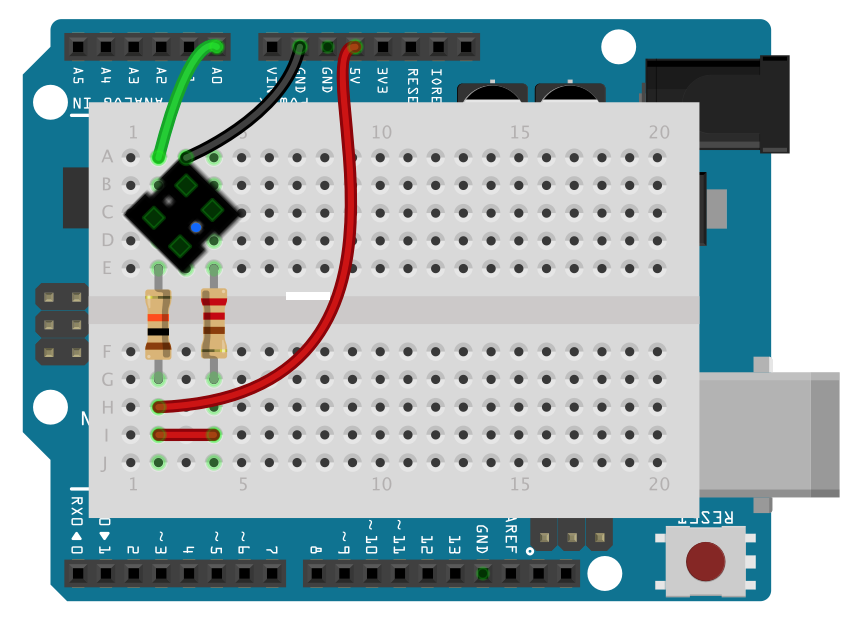
\includegraphics[width=0.45\textwidth]{Kapitel2/Bilder/cny70bb}
\caption{Aufbau der Schaltung}
\label{fig:cny70breadboard}
\end{center}
\end{figure}



\subsection{Aufgaben}
\subsubsection{Aufgabe 1}
In Abb. \ref{fig:cny70breadboard} ist eine funktionierende Schaltung abgebildet. Baue diese Schaltung nach, überprüfe zunächst die Funktion der IR-LED mit Hilfe einer Digitalkamera (z.B. deiner Smartphone-Camera\footnote{Neuere Smartphones funktionieren nicht, da oft die Camera einen guten IR-Filter besitzt}).  Wenn dieser Teil der Schaltung  funktioniert, dann kann die restliche Schaltung aufbauen werden. Achte besonders darauf keinen Kurzschluss zu verursachen und die richtigen Widerstände zu benutzen.

Lade anschließend den Sketch \ref{lst:tcny70} auf den Arduino und überprüfe mit Hilfe der seriellen Schnittstelle die Funktion deiner Schaltung.

\subsubsection{Aufgabe 2}
Um den Sketch voll zu nutzen müsst du deine Schaltung so umbauen, dass die IR-LED über den digitalen PIN 05 mit Spannung versorgt werden kann. 

Untersucht nun den Einfluss des Umgebungslichtes auf deine Messergebnisse. Wie kannst du den Einfluss reduzieren. (Physikalische aber auch programmtechnische Lösungen sind möglich)

\subsubsection{Aufgabe 3}
Versucht mit Hilfe deiner Schaltung eine schwarze Linie zu erkennen, indem du deine Schaltung über das Papier bewegt und die entsprechenden Werte für weißes Papier bzw. schwarze Linie notierst. Wenn du nun mit dem Reflexoptokoppler über eine schwarze Linie fährst, soll eine grüne LED aufleuchten. 


\clearpage


%%%%%%%%%%%%%%%%%%%%%%%%%%%%
%%%  Ultraschall       %%%%%
%%%%%%%%%%%%%%%%%%%%%%%%%%%%
\section{Digitaler Sensor: Der Ultraschallsensor}
\label{sec:ultra}
Ein Ultraschallsensor, wie der ''Seeed Ultrasonic Sensor'' von Seeed oder ''Ping))) Ultrasonic Range Sensorist'' von Parallax soll unser erstes Beispiel für einen digitaler Sensor sein. Wenn du die Rückseite des Sensors anschaust, dann siehst du sehr viel Elektronik und man ahnt schon, dass dieser Sensor wohl anderst funktioniert als z.B. ein Photowiderstand. 
\marginimage{Kapitel2/Bilder/Ping))}

\subsection{Funktionsweise des Ultraschallsensors}

\margininfo{Die Steuerung des Sensors und das Empfangen von Daten über digitale Pins wird auch Protokoll genannt! Im Falle des Ultraschallsensors ist das verwendete Protokoll aber sehr einfach. Das Protokoll, das wahrscheinlich am öftesten verwendet wird ist ``IPv4''. ``IPv4'' regelt LAN oder W-LAN Verbindung zwischen elektronischen Geräten.}

\begin{figure}[h]
\begin{center}
  \begin{tikzpicture}[remember picture]
    % Image 
    \node[anchor=south west,inner sep=0] (image) at (0,0) {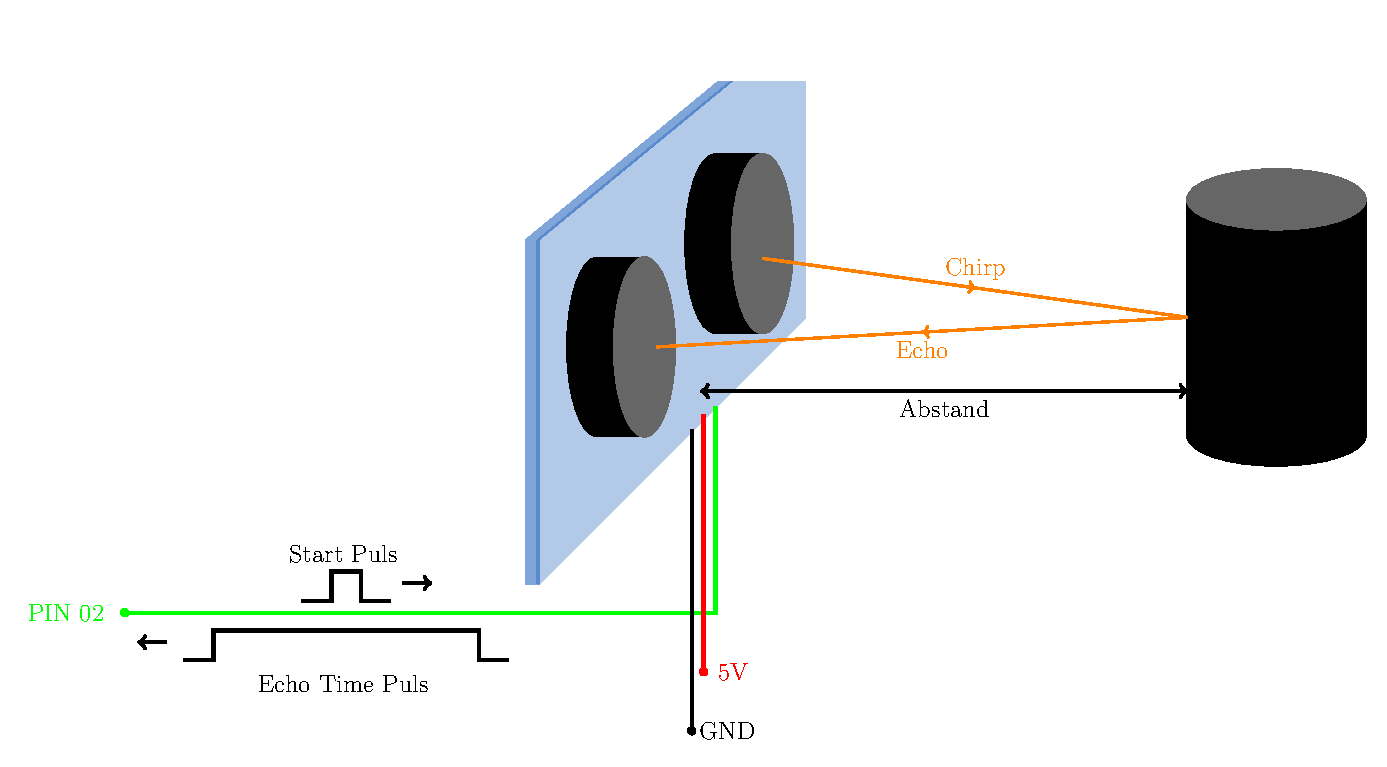
\includegraphics[width=0.9\textwidth]{Kapitel2/Bilder/funktPing}};
    
    % Marks 
    \node (start) at (4.5,3) {};
    \node (sender) at (9.5,6.5) {};
    \node (object) at (15,5.5) {};
    \node (collector) at (8,5) {};
    \node (signal) at (4,0.75) {};
    % comment
    \node[draw=red, fill=red!20, rounded corners,minimum width=0.2\textwidth, minimum height=1.4\baselineskip, anchor=west,align=center,text width=0.3\textwidth] (item1) at (0,4) {Messung wird durch den Startpuls begonnen};
    \node[draw=red, fill=red!20, rounded corners,minimum width=0.2\textwidth, minimum height=1.4\baselineskip, anchor=west,align=center,text width=0.3\textwidth] (item2) at (10,8){Sender: ein kurzer Ultraschall Plus wird ausgesendet};
    \node[draw=red, fill=red!20, rounded corners,minimum width=0.2\textwidth, minimum height=1.4\baselineskip, anchor=west,align=center,text width=0.2\textwidth] (item3) at (14,2.5){Gegenstand: Ultraschallpuls wird reflektiert};
    \node[draw=red, fill=red!20, rounded corners,minimum width=0.2\textwidth, minimum height=1.4\baselineskip, anchor=west,align=center,text width=0.2\textwidth] (item4) at (9.5,1.5){Empfänger: Reflektierter Ultraschallpuls wird erkannt};
    \node[draw=red, fill=red!20, rounded corners,minimum width=0.2\textwidth, minimum height=1.4\baselineskip, anchor=west,align=center,text width=0.4\textwidth] (item5) at (0,-0.5){Signal: Dauer des Antwortpulses entspricht der Flugzeit des Ultraschall Pulses};
    
    \path[red, thick,-] (start.south) edge [out=90 , in=-90] (item1);
    \path[red, thick,-] (sender.east) edge [out=0 , in=-90] (item2);
    \path[red, thick,-] (object.north) edge [out=-10 , in=90] (item3);
    \path[red, thick,-] (collector.north) edge [out=-20 , in=90] (item4);
    \path[red, thick,-] (signal.north) edge [out=-90 , in=90] (item5);
    
    
    \path[red, very thick,-latex'] (item1.north) edge [out=90, in=180](item2.west);
    \path[red, very thick,-latex'] (item2.east) edge [out=0 , in=30] (item3.east);
    \path[red, very thick,-latex']  (item3.south) edge [out=-90, in=0] (item4.east);
    \path[red, very thick,-latex']  (item4.south) edge [out=-90, in=0](item5.east);
    % grid 
    %\draw[color=red,help lines,xstep=1,ystep=1] (0,0) grid (18,8);
    %\draw[help lines,thin,xstep=.5,ystep=.5] (0,0) grid (18,8);
    %\foreach \x in {0,1,...,18} { \node [anchor=north] at (\x,0) {\x}; }
    % \foreach \y in {0,1,...,8} { \node [anchor=east] at (0,\y) {\y}; }  
  \end{tikzpicture}
  \end{center}
  \caption{Funktionsweise eines Untraschallsensors}
  \label{fig:funktPing}
\end{figure}

%Der Ultraschallsensor strahlt zyklisch einen kurzen, hochfrequenten Schallimpuls aus. Dieser pflanzt sich mit Schallgeschwindigkeit in der Luft fort. Trifft er auf ein Objekt, wird er dort reflektiert und gelangt als Echo zurück zum Ultraschallsensor. Aus der Zeitspanne zwischen dem Aussenden des Schallimpulses und dem Empfang des Echosignals berechnet der Ultraschallsensor intern die Entfernung zum Objekt. Da die Entfernung zum Objekt über eine Schall-Laufzeitmessung und nicht über eine Intensitätsmessung bestimmt wird, haben Ultraschallsensoren eine ausgezeichnete Hintergrundausblendung. Ultraschallsensoren erlauben Entfernungsmessungen von 20 mm bis 10 m und können dank der Laufzeitmessung den Messwert mit millimetergenauer Auflösung erfassen. 




\subsection{Beispiel Sketch}

\marginfigure{Kapitel2/Bilder/ping}{Ultraschall Sensor Ping)))}{fig:ping}

\begin{multicols}{2}
\begin{arduinoCode}{Testsketch für einen UltraschallSensor}{lst:ultra}
int pingPin = 2; (*@ \tikzmark{senPin} @*)

void setup() {
  Serial.begin(9600); 
}

void loop() {
  pinMode(pingPin, OUTPUT);  (*@ \tikzmark{output} @*)
  digitalWrite(pingPin, LOW);
  delayMicroseconds(2);
  digitalWrite(pingPin, HIGH); (*@ \tikzmark{startPuls} @*)
  delayMicroseconds(15);
  digitalWrite(pingPin, LOW);
  delayMicroseconds(20);
  
  
  pinMode(pingPin, INPUT);  (*@ \tikzmark{input} @*)
  long cm = pulseIn(pingPin, HIGH)/29/2; (*@ \tikzmark{echoPuls} @*)

  Serial.print(cm);
  Serial.println(" cm");
  
  delay(100);
}
\end{arduinoCode}
\vfill\null 
\columnbreak
\null\vfill 
\begin{itemize}
  \itemsep15pt
  \item[] \tikzmarkcomment{item1}{Digitaler PIN02 ist der Signal-Pin}
  \itemsep50pt
  \item[] \tikzmarkcomment{item2}{PIN02 wird auf ``OUTPUT'' gesetzt}
  \itemsep15pt
  \item[] \tikzmarkcomment{item3}{Start Puls wird gesendet}
  \itemsep25pt
  \item[] \tikzmarkcomment{item4}{PIN02 wird auf ``INPUT'' gesetzt}
  \itemsep35pt
  \item[] \tikzmarkcomment{item5}{Die Pulsdauer wird mit Hilfe der Funktion ``pulsIn()'' gemessen und mit Hilfe der Schallgeschwindigkeit in cm umgerechnet}
  \itemsep15pt
\end{itemize}
\vfill \null

\begin{tikzpicture}[remember picture,overlay]
  \path[red, thick,-] (senPin.east) edge [out=0 , in=180] (item1);
  \path[red, thick,-] (output.east) edge [out=0 , in=180] (item2);
  \path[red, thick,-] (startPuls.east) edge [out=0 , in=180] (item3);
  \path[red, thick,-] (input.east) edge [out=0 , in=180] (item4);
  \path[red, thick,-] (echoPuls.east) edge [out=-20 , in=180] (item5);
\end{tikzpicture}

\end{multicols}

\subsection{Aufgaben}

\margininfo{Um das Datenblatt im Internet zu finden, verwendest du die Suchwörter ``Datasheet'' und die Bezeichnung des Sensors}

Es gibt auch Ultraschallsensoren mit vier Beinchen. Dabei wird ein Pin zum senden des Start Pulses verwendet und der andere zum empfangen des Echo Pulses. Schreibe deinen Sketch so um, dass du den HC-SR04 Sensor verwenden kannst. Diese Sensoren sind um den Faktor fünf billiger als die mit drei Beinchen.
Finde anhand des Datenblattes zu deinem Ultraschallsensor den Messbereich und die Genauigkeit des Ultraschallsensors heraus. Baue dann die Schaltung entsprechend Abb. \ref{fig:ping} oder \ref{fig:hc-sr04} auf. Du muss unbedingt die Bezeichnung der Pins auf dem Sensor beachten, alle  Pins müssen richtig verbunden sein, ansonsten kann der Sensor zerstört werden (und die sind leider teuer).

\subsubsection{Aufgabe 1}
Lade den Sketch aus Listing \ref{lst:ultra} auf deinen Arduino und ändere ihn gegebenenfalls ab. Mach dich mit der Funktion vertraut und überprüfe den Messbereich und die Genauigkeit des Sensors. 

\marginfigure{Kapitel2/Bilder/ping-hc-sr04}{Ultraschall Sensor HC-SR04}{fig:hc-sr04}

                          
\subsubsection{Aufgabe 2}
Bau einen Ultraschallsensor und drei farbige LEDs (grün, gelb und rot) auf dein BreadBoard. Schreibe einen Sketch der einen optischen Abstandsmelder realisiert.

\begin{multicols}{2}
\begin{arduinoCode}{Testsketch "hc-sr04Test.ino" für den HC-SR04}{lst:hc-sr04}
int trigPin = 3; (*@ \tikzmark{trigPin} @*)
int echoPin = 2; (*@ \tikzmark{echoPin} @*)

void setup() { 
  Serial.begin(9600);
  pinMode(trigPin, OUTPUT); 
  pinMode(echoPin, INPUT); 
}

void loop() {
  digitalWrite(trigPin, HIGH); 
  delay(1000);                   (*@ \tikzmark{startPuls} @*)
  digitalWrite(trigPin, LOW);

  long cm = pulseIn(echoPin, HIGH)/29.1/2;(*@ \tikzmark{echoPuls} @*)
}
\end{arduinoCode}
\vfill\null 
\columnbreak
\null\vfill 
\begin{itemize}
  \itemsep15pt
  \item[] \tikzmarkcomment{item1}{Digitaler PIN02 ist der Trigger-Pin}
  \item[] \tikzmarkcomment{item2}{Digitaler PIN02 ist der Echo-Pin}
  \itemsep45pt
  \item[] \tikzmarkcomment{item3}{PIN02 wird auf auf HIGH gesetzt um den Start Puls zu senden}
  \itemsep35pt
  \item[] \tikzmarkcomment{item4}{Die Pulsdauer wird mit Hilfe der Funktion ``pulsIn()'' gemessen und mit Hilfe der Schallgeschwindigkeit in cm umgerechnet}
  \itemsep15pt
\end{itemize}
\vfill \null

\begin{tikzpicture}[remember picture,overlay]
  \path[red, thick,-] (trigPin.east) edge [out=0 , in=180] (item1);
  \path[red, thick,-] (echoPin.east) edge [out=0 , in=180] (item2);
  \path[red, thick,-] (startPuls.east) edge [out=0 , in=180] (item3);
  \path[red, thick,-] (echoPuls.east) edge [out=-20 , in=180] (item4);
\end{tikzpicture}

\end{multicols}

\clearpage

\section{Umwelt Sensoren}
\label{sec:UmweltSensoren}

Es gibt Sensoren, die so komplex sind, dass sie durch ein spezielles Protokoll gesteuert werden müssen. Für diese Sensoren ist dieses Protokoll in einer sogenannten Bibliothek (eng. Library) schon programmiert. Um den Snesor zu Benutzen wird am Anfang des Sketches diese mit Hilfe des Befehls ``\#include "libName.h";'' eingebunden. Dadurch wird der Befehlssatz des Arduino erweitert. Der Kombi-Sensor DH11 ist so ein Sensor. Er verbindet die Temperatur-Messung mit einer Feuchtigkeits-Messung der Luft. Mit Hilfe dieses Sensors kann der Taupunkt indirekt gemessen werden und so z.B. eine intelligente Raumlüftung realisiert werden, die effektive das kondensieren von Wasser an Wänden verhindert und so der Schimmelbindung aktiv entgegenwirkt. 



\marginfigure{Kapitel2/Bilder/dh11test}{Temperatur- und Feuchtigkeits-Sensor DH11}{fig:dh11test}

\subsection{Beispiel Sketch}

\begin{multicols}{2}
\begin{arduinoCode}{Test-Sketch für den DHT 11 Sensor}{lst:dht}
#include "DHT.h" (*@ \tikzmark{loadLib} @*)
          
DHT dht(6, DHT11); (*@ \tikzmark{object} @*)

void setup() {
  Serial.begin(9600); 
  dht.begin(); (*@ \tikzmark{begin} @*)
}

void loop() {
  delay(2000);

  float h = dht.readHumidity(); (*@ \tikzmark{readHumi} @*)
  float t = dht.readTemperature(); (*@ \tikzmark{readTemp} @*)
  
  if (isnan(h) || isnan(t)) { (*@ \tikzmark{check} @*)
    Serial.println("Failed to read!");
  } else {
    Serial.print("H= " + h + " % "); 
    Serial.print("T= " + t + " *C ");
  }  
}
\end{arduinoCode}
\vfill\null 
\columnbreak
\null\vfill 
\begin{itemize}
  \itemsep20pt
  \item[] \tikzmarkcomment{item1}{Zunächst wird die Bibliothek für den Seondor eingebunden}
  \itemsep25pt
  \item[] \tikzmarkcomment{item3}{Ein Sensor ``Objekt'' wird erzeugt}
  \item[] \tikzmarkcomment{item4}{Der Sensor wird gestartet, das dauert bis zu 2 Sekunden}
  \itemsep15pt
  \item[] \tikzmarkcomment{item5}{Das Auslesen der Luftfeuchtigkeit und Temperatur dauert jeweils 0,25 Sekunden! }
  \item[] \tikzmarkcomment{item6}{Ausgabe erfolgt nur, wenn das Lesen geklappt hat}
\end{itemize}
\vfill \null

\begin{tikzpicture}[remember picture,overlay]
  \path[red, thick,-] (loadLib.east) edge [out=0 , in=180] (item1);
  \path[red, thick,-] (object.east) edge [out=0 , in=180] (item3);
  \path[red, thick,-] (begin.east) edge [out=0 , in=180] (item4);
  \path[red, thick,-] (readHumi.east) edge [out=0 , in=180] (item5);
  \path[red, thick,-] (check.east) edge [out=0 , in=180] (item6);
  
\end{tikzpicture}

\end{multicols}

\subsection{Aufgaben}

Baue den DHT11 Sensor auf dem BreadBoard auf und teste deine Schlatung mit Hilfe des Beispielsketches.

\subsubsection{Aufgabe 1}
Schreibe ein Funktion vom Typ float, die als Parameter die Temperatur t und Luftfeuchtigkeit h besitzt und die Taupunkttemperatur $T_p$ berechnet.

\begin{equation}
  T_p = \left(\frac{h}{100}\right)^\frac{1}{8,02}(109,8+t)-109,8
\end{equation}

\begin{arduinoCode}{Taupunkttemperatur ``ttp''}{lst:ttp}
ttp = pow(H/100,1.0/8.02)*(109.8+t)+109.8;
\end{arduinoCode}

Erweitere deinen Sketch, so dass die Taupunkttemperatur berechnet wird und wenn die aktuellen Temperatur kleiner als die Taupunkttemperatur wird eine Warnung über die serielle Schnittstelle versendet wird.
 
\sectionExkurs{Daten Speichern und Auslesen}

\subsection{Die verschiedenen Speicher}
Auf dem Arduino Uno der ATmega328 Microcontroller verbaut. Er besitzt drei Arten von Steuer:
\begin{itemize}
  \item Flash ist der Speicher, in dem der Sketch gespeichert und ausgeführt wird. 
  \item SRAM ist der Speicher, in dem Variablen gespeichert und manipuliert werden können.
  \item EEPROM ist der Speicher, der von Programmen genutzt werden kann um Daten dauerhaft zu speichern.
\end{itemize}


Flash Speicher und  EEPROM Speicher sind nicht flüchtig, das heißt die Daten sind auch nach Stromunterbrechung noch vorhanden. SRAM Speicher ist flüchtig, das heißt die gespeicherten Daten sind nach einer Stromunterbrechung nicht mehr vorhanden. Der ATmega328 IC besitzt folgende Speichergrößen:

\begin{figure}[h]
  \begin{center}
  \tikzset{ 
      table/.style={
          matrix of nodes,
          row sep=-\pgflinewidth,
          column sep=-\pgflinewidth,
          nodes={
              rectangle,
              draw=black,
              align=center
          },
          minimum height=1.5em,
          text depth=0.5ex,
          text height=2ex,
          nodes in empty cells,
  %%
          every even row/.style={
              nodes={fill=gray!20}
          },
          column 1/.style={
              nodes={text width=0.1\textwidth}
          },
          column 2/.style={
              nodes={text width=0.1\textwidth}
          },
          column 3/.style={
              nodes={text width=0.4\textwidth}
          },
          row 1/.style={
              nodes={
                  fill=black!80,
                  text=white,
                  font=\bfseries
              }
          }
      }
  }
  \begin{tikzpicture}
  \matrix (first) [table,text width=6em]
  {   
   Speicher & Größe & Bemerkung \\
   Flash  & 32kB & 0.5kB enthält den Bootloader \\
   SRAM   & 2kB & Speicherbereich für Varaiablen\\
   EEPROM & 1kB & Langzeit Speicher\\
  };
  \end{tikzpicture}
  \caption{Speichergrößen des Arduino Uno}
  \label{tab:speicher}
  \end{center}
\end{figure}
\margininfo{1kB = 1024 Byte \\ B steht für Byte \\ ein Byte besteht aus 8 Bit \\ 1 Bit ist die kleinste Speichergröße}
Es gibt nicht wirklich viel SRAM auf dem Arduino Uno! Bei größeren Datenmengen kann es passieren, dass er vollständig gefüllt wird. Zum Beispiel
\begin{arduinoCode}{}{}
char message[] = "I support the Cape Wind project.";
\end{arduinoCode}
belegt 33 Bytes im SRAM, jedes Zeichen und das Endzeichen '\textbackslash 0' ein Byte.
Dies scheint nicht viel zusein, aber es braucht nicht viel um 2048 Bytes zu füllen. Wenn du den ganzen SRAM aufgebracht hast, kann es zu komischen Fehlern kommen.

Du kannst so eine Sketch oft ohne Fehler auf den Arduino laden, da der SRAM während der Laufzeit gefüllt wird. Wenn der Sketch dann ausgeführt werden soll funktioniert er nicht richtig. Es kommt du komischen Fehlern, die nur sehr schwer zu verstehen sind.

\subsection{EEPROM Speicher benutzen}

\begin{multicols}{2}
\begin{arduinoCode}{EEPROM mit Daten füllen}{lst:eeprom-write}
#include <EEPROM.h> (*@ \tikzmark{lib} @*) 

void setup()
{   (*@ \tikzmark{for} @*) 
  for (int i = 0; i < 255; i++)
    EEPROM.write(i, i); (*@ \tikzmark{write} @*) 
}

void loop()
{
}
\end{arduinoCode}

\vfill
\columnbreak

\null\vfill
\begin{itemize}
  \itemsep15pt
  \item[] \tikzmarkcomment{item1}{EEPROM Library einbinden}
  \item[] \tikzmarkcomment{item2}{for-Schleife}
  \item[] \tikzmarkcomment{item3}{Daten schreiben}
\end{itemize}
\vfill \null

\begin{tikzpicture}[remember picture,overlay]
  \path[red, thick,-] (lib.east) edge [out=0 , in=180] (item1);
  \path[red, thick,-] (for.east) edge [out=5 , in=180] (item2);
  \path[red, thick,-] (write.east) edge [out=0 , in=180] (item3);
\end{tikzpicture}

\end{multicols}


\begin{multicols}{2}
\begin{arduinoCode}{EEPROM mit Daten füllen}{lst:eeprom-write}
#include <EEPROM.h> (*@ \tikzmark{lib} @*) 

int a = 0;
int value;

void setup() {
  Serial.begin(9600);
}

void loop() {
  value = EEPROM.read(a); (*@ \tikzmark{read} @*) 

  Serial.print(a); (*@ \tikzmark{ser} @*) 
  Serial.print(" = ");
  Serial.println(value);
  
  a = a + 1; (*@ \tikzmark{ort} @*) 
  if (a == 256) {
    a = 0;
  }
  delay(500);
}
\end{arduinoCode}

\vfill
\columnbreak

\null\vfill
\begin{itemize}
  \itemsep15pt
  \item[] \tikzmarkcomment{item1}{EEPROM Library einbinden}
  \item[] \tikzmarkcomment{item2}{Daten aus EEPROM lesen}
  \item[] \tikzmarkcomment{item3}{Daten über serielle Schnittstelle an PC übertragen}
  \item[] \tikzmarkcomment{item4}{Leseort um eine Einheit erhöhen}
\end{itemize}
\vfill \null

\begin{tikzpicture}[remember picture,overlay]
  \path[red, thick,-] (lib.east) edge [out=0 , in=180] (item1);
  \path[red, thick,-] (read.east) edge [out=5 , in=180] (item2);
  \path[red, thick,-] (ser.east) edge [out=0 , in=180] (item3);
  \path[red, thick,-] (ort.east) edge [out=0 , in=180] (item4);
\end{tikzpicture}

\end{multicols}


%%%%%%%%%%%%%%%%%%%%%%%%%%%%%%%%%%%%%%%%%%%%%%%%%%%%%%%
%%%  Schleifen %%%%%%%%%%%%%%%%%%%%%%%%%%%%%%%%%%%%%%%%
%%%%%%%%%%%%%%%%%%%%%%%%%%%%%%%%%%%%%%%%%%%%%%%%%%%%%%%
\sectionInformatik{C Sprachstruktur: Schleifen}
Eine Schleife ist eine weitere Kontrollstruktur. Sie dient zur Wiederholung eines Anweisungsblock, den sogenannten Schleifenrumpf oder Schleifenkörper. Dieser wird solange die Schleifenbedingung als Laufbedingung gültig bleibt bzw. die Abbruchbedingung nicht eintritt wiederholt. Schleifen, die keine Schleifenbedingung haben, sind Endlosschleifen. Im Arduino-Sketch stellt die Loop-Methode eine solche Endlosschleife dar.

Prinzipiell können verschiedene Schleifentypen  unterschieden werden:
\begin{itemize}
  \item Die vorprüfende oder kopfgesteuerte Schleife. \\
    Bei dieser Schleife wird eine Bedingung geprüft, mit der vorher entschieden wird, ob der Schleifenkörper ausgeführt wird, diese wird meist als  while-Schleife bezeichnet.
  \item Die nachprüfende oder fußgesteuerte Schleife. \\
    Bei dieser Schleife wird nach dem Durchlauf des Schleifenkörpfers eine Bedingung überprüft, ob der Schleifenrumpf nochmal ausgeführt wird (meist als DO...WHILE = „ausführen...solange“ oder REPEAT...UNTIL = „wiederholen...bis“ Konstrukt).

  \item Die Zählschleife, eine Sonderform der vorprüfenden Schleife (meist als FOR = für -Schleife implementiert). \\
  \item Die Mengenschleife, eine Sonderform der Zählschleife (meist als FOREACH = „für jedes Element der Menge“ implementiert).
  \item Schleife mit Laufbedingung: Wertet die Bedingung zu „wahr“ aus, wird die Schleife fortgesetzt.
    Schleife mit Abbruchbedingung: Wertet die Bedingung zu „wahr“ aus, so wird die Schleife abgebrochen.
\end{itemize}

\marginfigure{Kapitel2/Tikz/out/for.pdf}{for-Loop}{fig:for-loop}

\subsection{for-Schleife: die zählende Wiederholung}

Eine for-Schleife ist eine Kontrollstruktur, mit der man eine Gruppe von Anweisungen, den Schleifenkörper mit einer bestimmten Anzahl von Wiederholungen ausführen kann.
Die Anzahl der Wiederholungen steht schon beim Eintritt in die Schleife fest. Es gibt eine Schleifenvariable, die am Anfang auf den Startwert gesetzt wird und dann jeweils um die Schrittweite verändert wird, bis der Zielwert erreicht ist. Die Schleifenvariable, der Startwert, die Schrittweite und der Endwert müssen numerisch sein. 

\begin{multicols}{2}
\begin{arduinoCode}{Die for-Schleife}{lst:forloop}

        (*@ \tikzmark{ini} @*)               (*@ \tikzmark{test} @*)
for (Initialisieren; Testen; Zaehlen) {
                              (*@ \tikzmark{inc} @*)

 // Anweisungen; (*@ \tikzmark{anw} @*)


}
\end{arduinoCode}

\vfill
\columnbreak

\begin{itemize}
  \itemsep15pt
  \item[] \tikzmarkcomment{item1}{Initialisieren der Schleifenvariablen}
  \item[] \tikzmarkcomment{item2}{Bedingung für die Schleifenvariablen überprüfen.}
  \item[] \tikzmarkcomment{item3}{Schleifenvariablen erhöhen}
  \item[] \tikzmarkcomment{item4}{Anweisungen, die wiederholt ausgeführt werden.}
\end{itemize}


\begin{tikzpicture}[remember picture,overlay]
  \path[red, thick,-] (ini.east) edge [out=35 , in=180] (item1);
  \path[red, thick,-] (test.east) edge [out=20 , in=180] (item2);
  \path[red, thick,-] (inc.east) edge [out=-5 , in=180] (item3);
  \path[red, thick,-] (anw.east) edge [out=-5 , in=180] (item4);
\end{tikzpicture}
\vfill 
\end{multicols}


In C ist die for-Schleife viel flexibler als for-Schleifen in vielen anderen Programmiersprachen, einschließlich BASIC. So kann auf alle der drei Kopfelemente verzichtet werden, nur die Strichpunkte sind nötig. 

 

\clearpage
\subsubsection{Sensorwert in Array speichern und Mittelwert berechnen}

\begin{multicols}{2}
\begin{arduinoCode}{Mittelwert berechnen}{lst:calcMean}
const int senPin = A0;
const int numberOfValues = 10; (*@ \tikzmark{number} @*)
float senValues[numberOfValues]; (*@ \tikzmark{sensorValues} @*) 
float meanValue = 0.0; (*@ \tikzmark{meanValue} @*)

void setup() {
  Serial.begin(9600);
  
}

void loop() {
  for (int i=0;i<numberOfValues;i++) { (*@ \tikzmark{measureLoop} @*)
    senValues[i] = analogRead(senPin);
    delay(20);
  }
  for (int i=0;i<numberOfValues;i++) { (*@ \tikzmark{meanLoop} @*)
     meanValue += senValues[i];
  }
  
  meanValue /= numberOfValues; (*@ \tikzmark{calcMean} @*)
  Serial.println(meanValue);
  delay(200);  
}
\end{arduinoCode}
\vfill
\columnbreak
\null\vfill
\begin{itemize}
  \itemsep25pt
  \item[] \tikzmarkcomment{item1}{Anzahl der Einzelmessungen}
  \item[] \tikzmarkcomment{item2}{Array zur Speicherung der Einzelmessungen}
  \item[] \tikzmarkcomment{item3}{Speicherplatz für gemittelten Sensorwert.}
  \item[] \tikzmarkcomment{item4}{Loop für die Einzelmessungen}
  \item[] \tikzmarkcomment{item5}{Loop für die Mittelwertbildung}
  \item[] \tikzmarkcomment{item6}{Mittelwert berechnen und an PC senden}
\end{itemize}
\vfill \null
\begin{tikzpicture}[remember picture,overlay]
  \path[red, thick,-] (number.east) edge [out=0 , in=180] (item1);
  \path[red, thick,-] (sensorValues.east) edge [out=0 , in=180] (item2);
  \path[red, thick,-] (meanValue.east) edge [out=0 , in=180] (item3);
  \path[red, thick,-] (measureLoop.east) edge [out=0 , in=180] (item4);
  \path[red, thick,-] (meanLoop.east) edge [out=0 , in=180] (item5);  
  \path[red, thick,-] (calcMean.east) edge [out=0 , in=180] (item6);  
\end{tikzpicture}
\end{multicols}

\subsection{Aufgaben}

\subsubsection{Aufgabe 1} 
Schreibe einen Sketch, der die Summe der ganzen Zahlen von 1 bis 10 berechnet. Gib dein Ergebnis über die serielle Schnittstelle aus.


\clearpage 
\subsection{while-Schleife: die bedingte Wiederholung}



\marginfigure{Kapitel2/Tikz/out/while.pdf}{while-Loop}{fig:while-loop}
\begin{multicols}{2}
\begin{arduinoCode}{Die for-Schleife}{lst:forloop}

           (*@ \tikzmark{test} @*)
 while (bedingung) {
   
 // Anweisungen; (*@ \tikzmark{anw} @*)

}
\end{arduinoCode}

\vfill
\columnbreak

\begin{itemize}
  \itemsep15pt
  \item[] \tikzmarkcomment{item1}{Bedingung auf Wahrheit  überprüfen.}
  
  \item[] \tikzmarkcomment{item2}{Anweisungen, die wiederholt ausgeführt werden.}
\end{itemize}


\begin{tikzpicture}[remember picture,overlay]
  \path[red, thick,-] (test.east) edge [out=20 , in=180] (item1);
  \path[red, thick,-] (anw.east) edge [out=-5 , in=180] (item2);
\end{tikzpicture}
\vfill 
\end{multicols}


\subsection{Sprungbefehle}

Möchte man innerhalb einer Schleife (for, do oder while) auf ein Ereignis reagieren, indem die Schleife nicht weiter ausgeführt wird, steht der Befehl break zur Verfügung. Sprungbefehle sollte aber nur dann benutzt werden, wenn es keine andere Lösung gibt (, was praktisch nie der Fall ist).



\begin{multicols}{2}
\begin{arduinoCode}{MVerwendung von break}{lst:break}
for (x = 0; x < 255; x ++)
{
    analogWrite(pwmPin, x);
    sens = analogRead(sensorPin);  
    if (sens > threshold){ 
       x = 0;
       break;  (*@ \tikzmark{break} @*)
    }  
    delay(50);
}
(*@ \tikzmark{cont} @*)

\end{arduinoCode}
\vfill
\columnbreak
\null\vfill
\begin{itemize}
  \itemsep35pt
  \item[] \tikzmarkcomment{item1}{Wenn ein bestimmter Sensorwert überschritten ist, dann wird mit Hilfe des Befehls Break das weiter abarbeiten der for-Schleife unterrochen}
  \item[] \tikzmarkcomment{item2}{und der Sketch nach dem Ende des Schleifenkörpers sortgesetzt}
\end{itemize}
\vfill \null
\begin{tikzpicture}[remember picture,overlay]
  \path[red, thick,-] (break.east) edge [out=0 , in=180] (item1);
  \path[red, thick,-] (cont.east) edge [out=0 , in=180] (item2);  
\end{tikzpicture}
\end{multicols}










